% ============================================================
% 北向资金对A股市场的影响与基于北向资金的量化交易策略 — 答辩PPT
% 编译方式：XeLaTeX（推荐）或 LuaLaTeX
% 在 VSCode 中使用 LaTeX Workshop 插件，选择 xelatex 编译链即可
% ============================================================
\documentclass[aspectratio=169, 10pt]{beamer}

% ---------- 中文支持 ----------
\usepackage{ctex}

% ---------- 主题与配色 ----------
\usetheme{Madrid}
\usecolortheme{seahorse}
\setbeamertemplate{navigation symbols}{}          % 去掉导航按钮
\setbeamertemplate{footline}[frame number]         % 仅显示页码

% ---------- 常用宏包 ----------
\usepackage{graphicx}
\usepackage{booktabs}
\usepackage{amsmath,amssymb}
\usepackage{tabularx}

% ---------- 图片路径 ----------
\graphicspath{{../Figure/}{./}}

% ============================================================
\title{北向资金对A股市场的影响\\与基于北向资金的量化交易策略}
\author{杨明宸}
\institute{清华大学}
\date{\today}
% ============================================================

\begin{document}

% ======================== 封面 ========================
\begin{frame}
\titlepage
\end{frame}

% ======================== 目录 ========================
\begin{frame}{报告提纲}
\tableofcontents
\end{frame}

% ======================== 第一部分：研究背景与目标 ========================
\section{研究背景与目标}

\begin{frame}{研究背景与目标}
\textbf{背景}
\begin{itemize}
    \item 沪港通2014年开通以来，北向资金规模与市场影响力持续扩大；日均成交占比10\%--15\%。
    \item 市场普遍将北向资金默认为"聪明钱"，但缺乏严谨的实证支持；现有文献结论相互矛盾。
\end{itemize}

\vspace{0.5em}
\textbf{学术目标}——回答三组核心问题：
\begin{enumerate}
    \item 北向资金是否具备显著超额收益？收益来源是选股还是择时？
    \item 北向资金净流入是否引发A股市场羊群效应？
    \item 允许北向资金交易是否系统性地改变个股波动率？
\end{enumerate}

\vspace{0.3em}
\textbf{工业目标}：构建基于北向资金信息的、与动量反转策略正交的高质量可交易alpha。

\vspace{0.3em}
\textbf{数据}：沪市A股，2017年10月--2025年10月，个股日度持仓与行情数据。
\end{frame}

% ======================== 第二部分：北向资金自身特征 ========================
\section{北向资金自身特征}

\begin{frame}{结论一：北向资金具备显著超额收益}
\begin{columns}[T]
\column{0.52\textwidth}
\begin{itemize}
    \item 构建\textbf{修正相关系数} $\widetilde{Corr}_t$（省略截面去均值化，同时捕捉选股+择时收益）。
    \item HAC稳健$t$检验：$\hat{\alpha}=0.0021$，$t=3.82$，\textbf{在1\%水平下高度显著}。
    \item 北向资金主动交易产生的累计相对收益在扣除多种费率情景后依然稳健上升。
\end{itemize}
\column{0.46\textwidth}
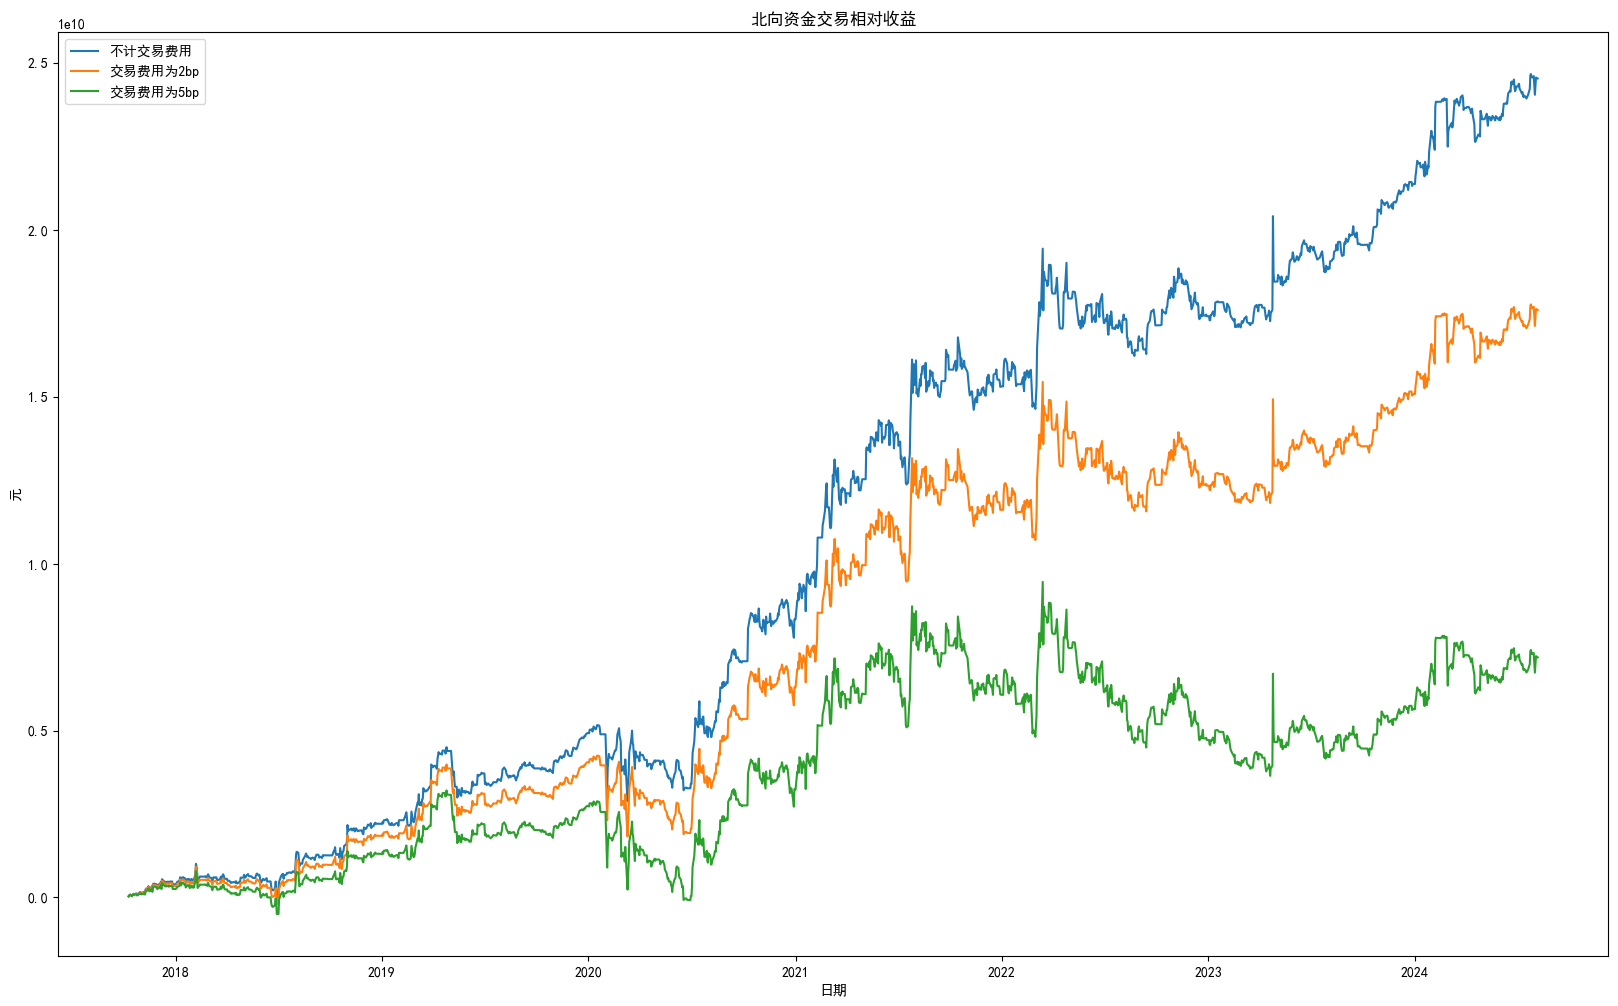
\includegraphics[width=\linewidth]{北向交易相对收益.png}
{\scriptsize 图：北向资金主动交易累积相对收益（多费率情景）}
\end{columns}
\end{frame}

\begin{frame}{结论二：择时贡献58\%，选股贡献42\%}
\begin{columns}[T]
\column{0.52\textwidth}
\begin{itemize}
    \item 将总收益分解为\textbf{选股收益}（CsPnl）与\textbf{择时收益}（TsPnl）。
    \item 择时收益累计金额更高（57.66\%），但选股收益夏普比率更优（1.04 vs 0.82）。
    \item \textbf{核心结论}：北向资金的信息优势更多体现在对市场短期涨跌方向的把握上。
\end{itemize}

\vspace{0.3em}
{\small
\begin{tabular}{lcc}
\toprule
\textbf{收益类型} & \textbf{年化Sharpe} & \textbf{贡献度} \\
\midrule
选股收益 & 1.04 & 42.34\% \\
择时收益 & 0.82 & 57.66\% \\
\midrule
总收益 & 1.38 & --- \\
\bottomrule
\end{tabular}
}

\column{0.46\textwidth}
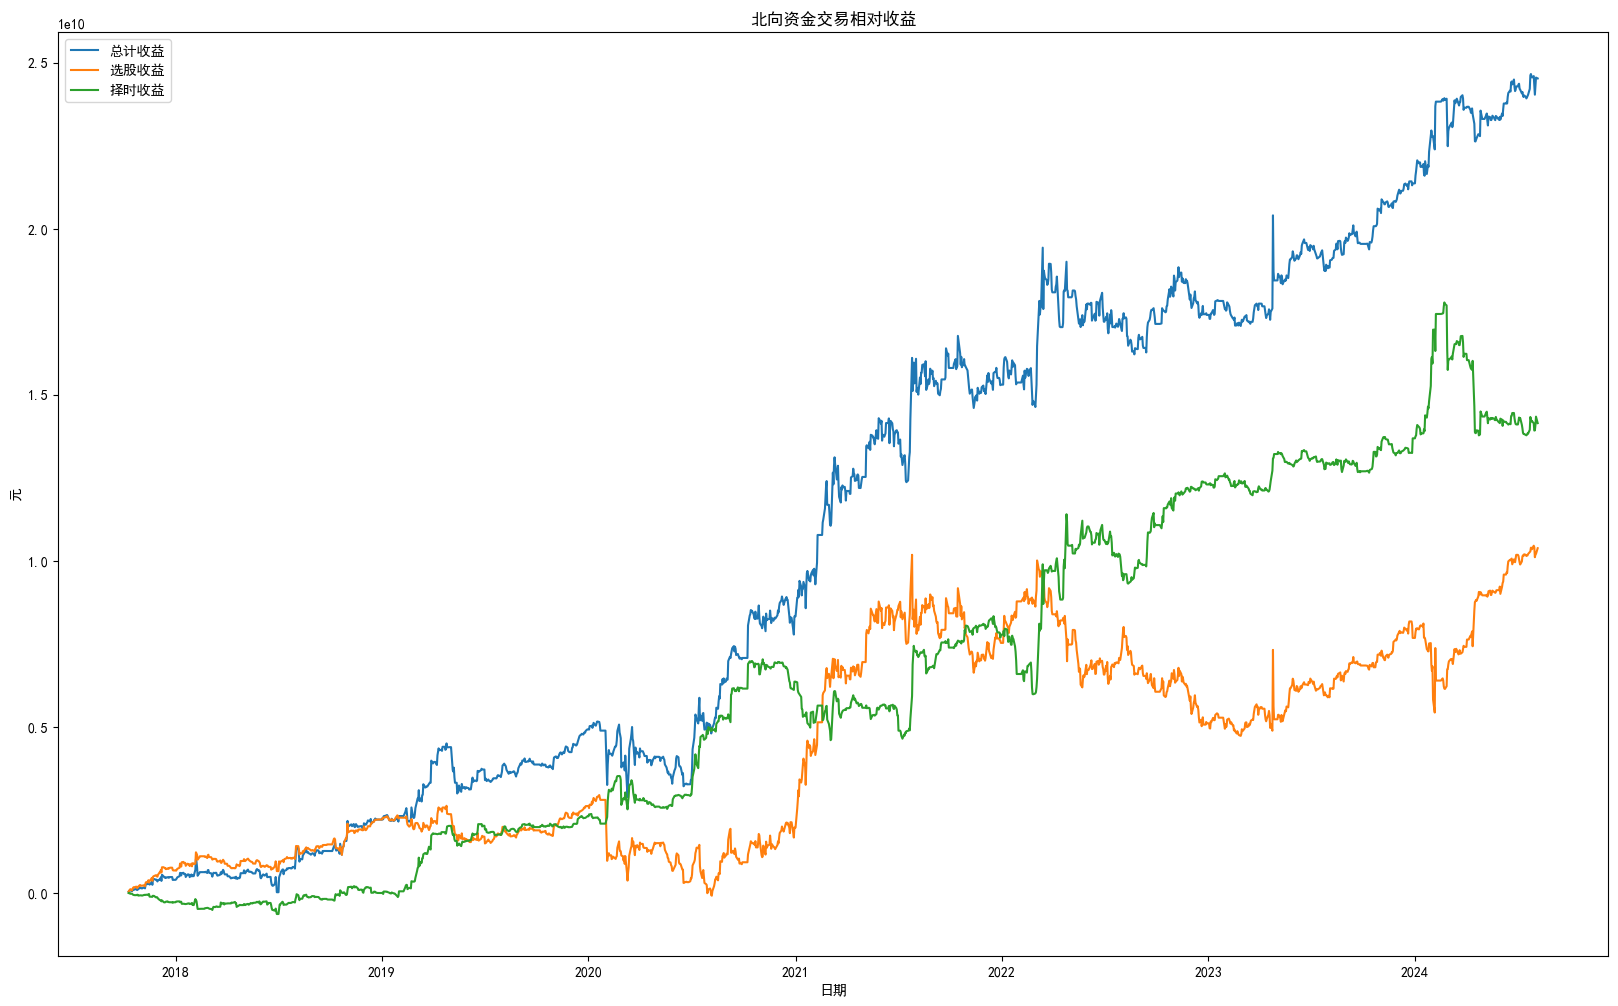
\includegraphics[width=\linewidth]{收益分解.png}
{\scriptsize 图：选股收益与择时收益累计曲线}
\end{columns}
\end{frame}

\begin{frame}{结论三：高频交易特征 \& 仅具短期预测能力}
\begin{columns}[T]
\column{0.52\textwidth}
\textbf{交易模式}
\begin{itemize}
    \item 构造适配非对称买卖结构的交易率指标。
    \item 北向资金日换手率\textbf{远超}内地机构，接近散户水平——"对冲基金式"高频交易特征。
\end{itemize}

\vspace{0.4em}
\textbf{预测期限递减}
\begin{itemize}
    \item 日频 $t=3.82^{***}$；1月 $t=2.16^{**}$；
    \item 半年 $t=0.53$；1年 $t=-0.24$。
    \item \textbf{结论}：信息优势高度集中于极短期价格波动，长期预测力趋零。
\end{itemize}

\column{0.46\textwidth}
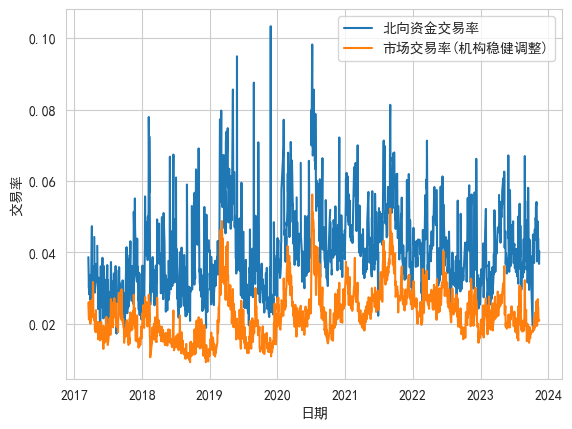
\includegraphics[width=\linewidth]{turnover_2.png}
{\scriptsize 图：北向资金换手率 vs 全市场换手率（调整后）}
\end{columns}
\end{frame}

% ======================== 第三部分：北向资金对A股的影响 ========================
\section{北向资金对A股市场的影响}

\begin{frame}{结论四：羊群效应——持续约一周}
\begin{columns}[T]
\column{0.52\textwidth}
\begin{itemize}
    \item 使用\textbf{VAR(4)模型}+格兰杰因果检验+脉冲响应函数。
    \item 北向净流入 $\to$ A股成交额：$F=15.44$，$p<0.001$。
    \item 反向因果较弱：$F=4.204$，$p=0.002$。
    \item \textbf{脉冲响应}：北向净流入冲击后，成交额在4个交易日内显著为正响应，之后衰减。
    \item \textbf{结论}：北向资金通过信号释放与媒体传播引发约\textbf{一周}的内地投资者跟风交易。
\end{itemize}

\column{0.46\textwidth}
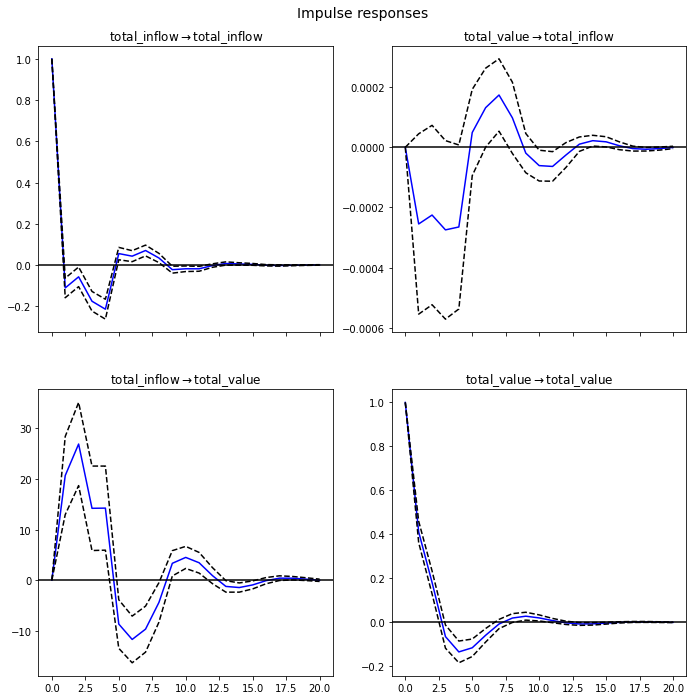
\includegraphics[width=\linewidth]{irf_value.png}
{\scriptsize 图：双向脉冲响应函数（20阶）}
\end{columns}
\end{frame}

\begin{frame}{结论五：沪港通开通导致标的股波动率系统性上升（DID）}
\begin{columns}[T]
\column{0.55\textwidth}
\begin{itemize}
    \item \textbf{准自然实验}：2014.11.17沪港通开通；实验组467只标的股 vs 对照组280只非标的股。
    \item 双重差分法（DID），控制个体固定效应+时间固定效应。
    \item 核心系数 $\hat{\beta}_3$（Post $\times$ Experiment）在6组回归中\textbf{均在1\%水平下显著为正}，且点估计高度稳定。
    \item 剔除事件前后各1个月数据后结论依然稳健$\Rightarrow$排除暂时性效应。
\end{itemize}

\vspace{0.3em}
\textbf{结论}：北向资金交易准入\textbf{系统性地提高}了标的股票的收益波动率。

\column{0.43\textwidth}
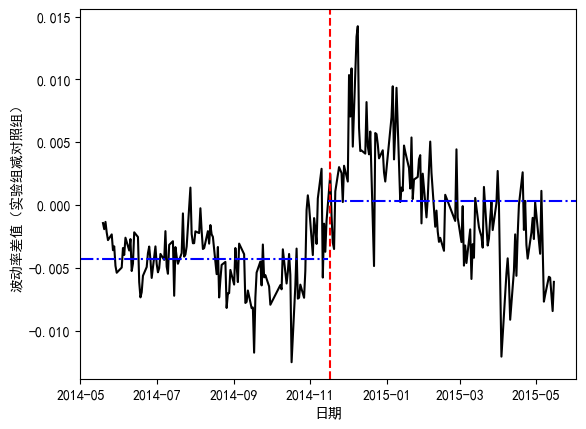
\includegraphics[width=\linewidth]{vol_1.png}
{\scriptsize 图：实验组与对照组波动率差值（Vol$_1$）}

\vspace{0.3em}
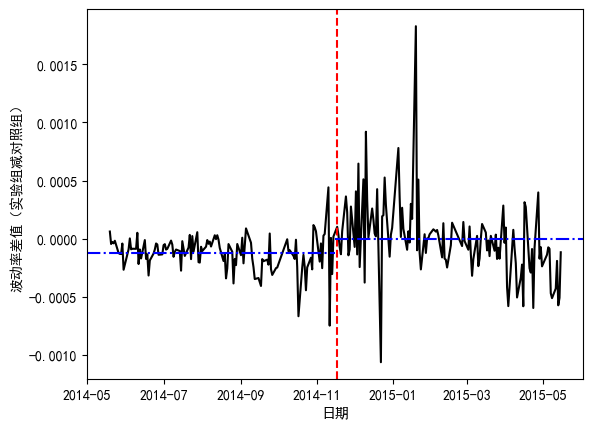
\includegraphics[width=\linewidth]{vol_2.png}
{\scriptsize 图：实验组与对照组波动率差值（Vol$_2$）}
\end{columns}
\end{frame}

% ======================== 第四部分：量化策略 ========================
\section{量化交易策略}

\begin{frame}{策略框架：解决A股虚假动量alpha问题}
\textbf{核心问题}：A股因卖空限制+涨跌停板，传统动量反转策略产生大量\textbf{不可交易的虚假alpha}。

\vspace{0.3em}
\textbf{解决方案}：构建"类Barra"残差化目标（bret），在训练目标层面预先剔除动量效应：
\begin{itemize}
    \item 在每日横截面上对原始回报率关于\textbf{1日/5日/21日/252日回报率 + log市值 + 行业哑变量}做OLS回归，取残差作为预测目标。
    \item 确保后续alpha与\textbf{所有滞后收益率的线性组合完全正交}。
\end{itemize}

\vspace{0.3em}
\textbf{特征工程}：26个特征，基于北向资金"持仓市值"与"净持仓变动"两个核心字段，采用多半衰期EMA（0.1/1/5/10日）+ ts-zscore/L2归一化 + 滞后回报率残差化 + RSI变体。

\vspace{0.3em}
\textbf{模型}：增量式滚动Ridge回归（每日在线更新），每天均为真正的样本外预测。
\end{frame}

\begin{frame}{结论六：线性模型样本外表现优异}
\begin{columns}[T]
\column{0.55\textwidth}
\textbf{核心指标}（样本外回测，2019--2025）：
\begin{itemize}
    \item 年化超额收益：\textbf{14.5\%}
    \item 年化夏普比率：\textbf{$\approx$ 5.0}
    \item 日均IC：\textbf{0.012}
    \item Alpha ACF半衰期：$\approx$ \textbf{0.88个交易日}——与北向资金高频交易特征吻合
\end{itemize}

\vspace{0.3em}
\textbf{关键性质}：
\begin{itemize}
    \item Alpha与所有动量反转策略在统计上\textbf{完全正交}——真正可交易。
    \item 累积平均SP单调上升，无长期回撤。
\end{itemize}

\column{0.43\textwidth}
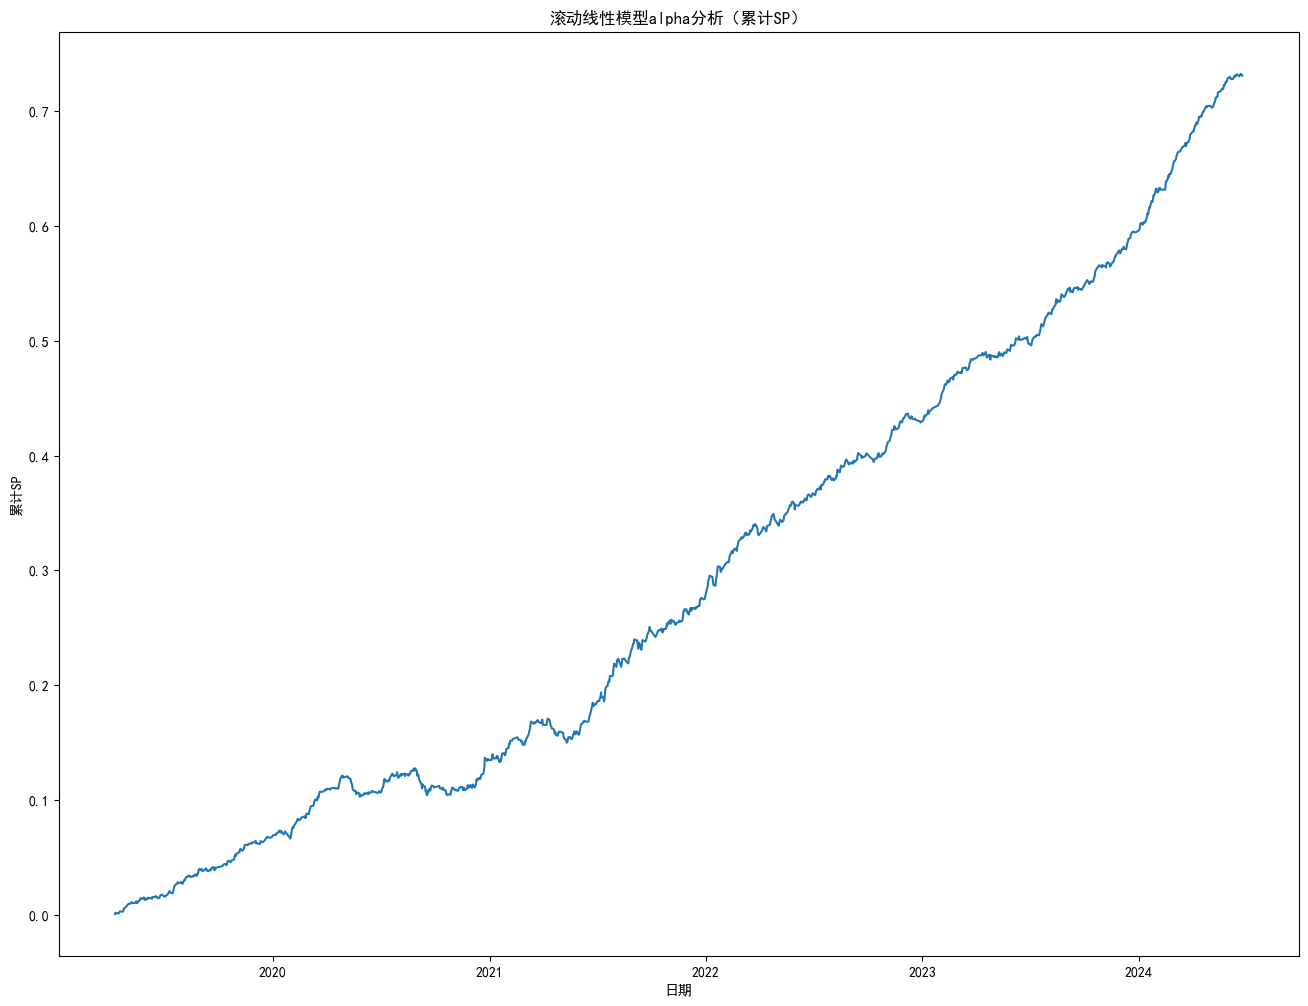
\includegraphics[width=\linewidth]{rollingWLS_SP.png}
{\scriptsize 图：累积平均SP曲线}

\vspace{0.3em}
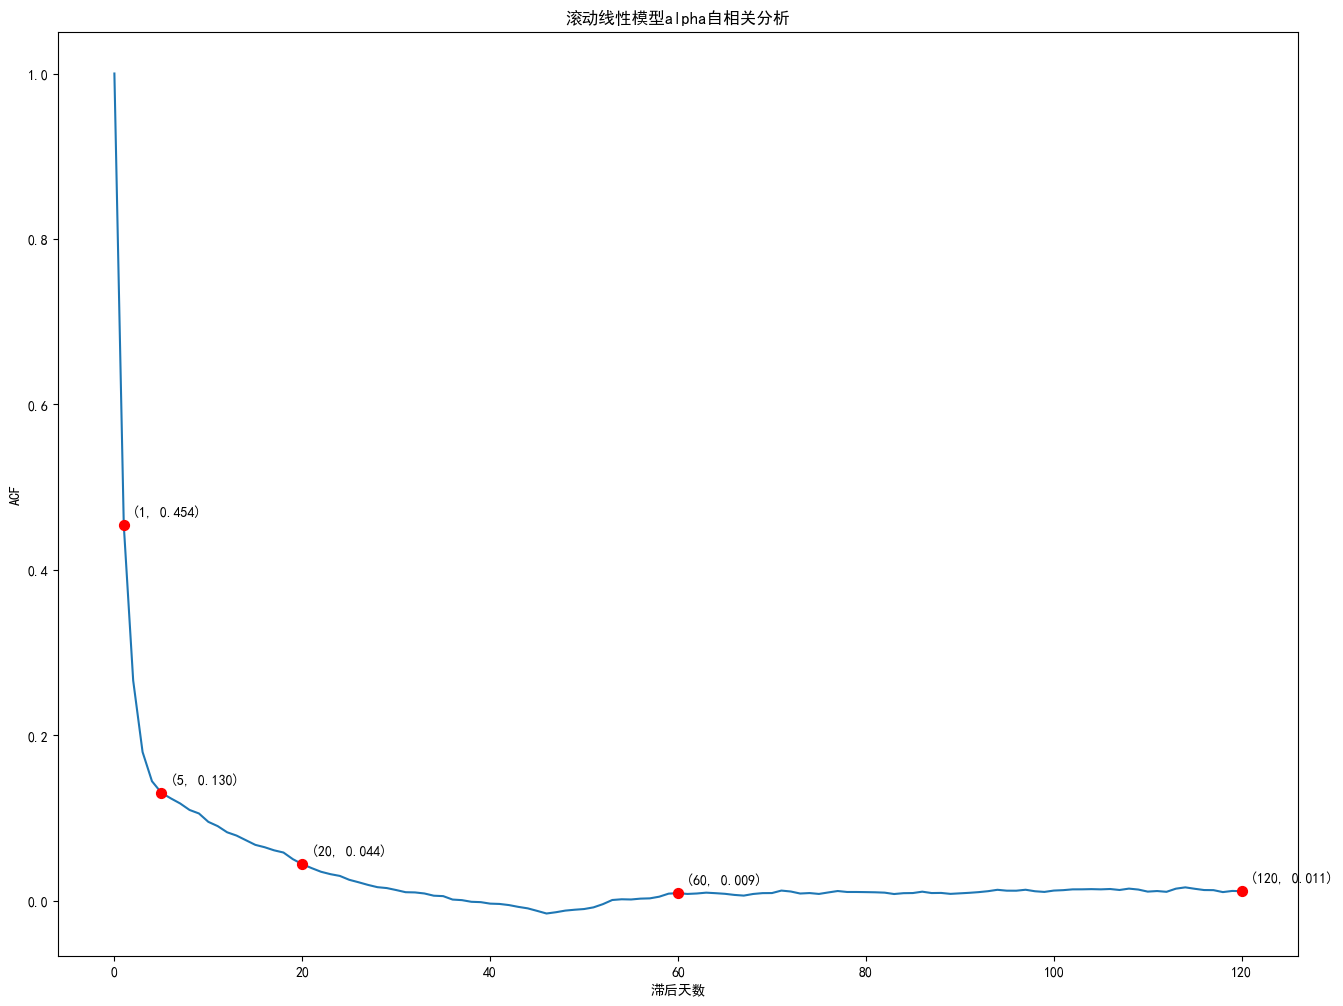
\includegraphics[width=\linewidth]{ACF.png}
{\scriptsize 图：Alpha信号自相关函数}
\end{columns}
\end{frame}

\begin{frame}{结论七：非线性模型无显著样本外增益}
\begin{columns}[T]
\column{0.52\textwidth}
\begin{itemize}
    \item 使用\textbf{LightGBM}与\textbf{CatBoost}两类GBDT模型。
    \item 样本内：非线性模型IC远高于线性基准（拟合容量更大）。
    \item \textbf{样本外}：IC增益几乎为零，与线性基准高度重叠。
\end{itemize}

\vspace{0.3em}
\textbf{原因分析}：
\begin{itemize}
    \item 残差化后信噪比极低（IC$\approx$0.012）
    \item 26个特征均基于两个核心字段派生，独立维度有限
    \item 有效独立样本量不足以支撑非线性模型的参数空间
\end{itemize}

\vspace{0.3em}
\textbf{结论}：当前特征框架下alpha的可预测成分\textbf{主要为线性结构}。

\column{0.46\textwidth}
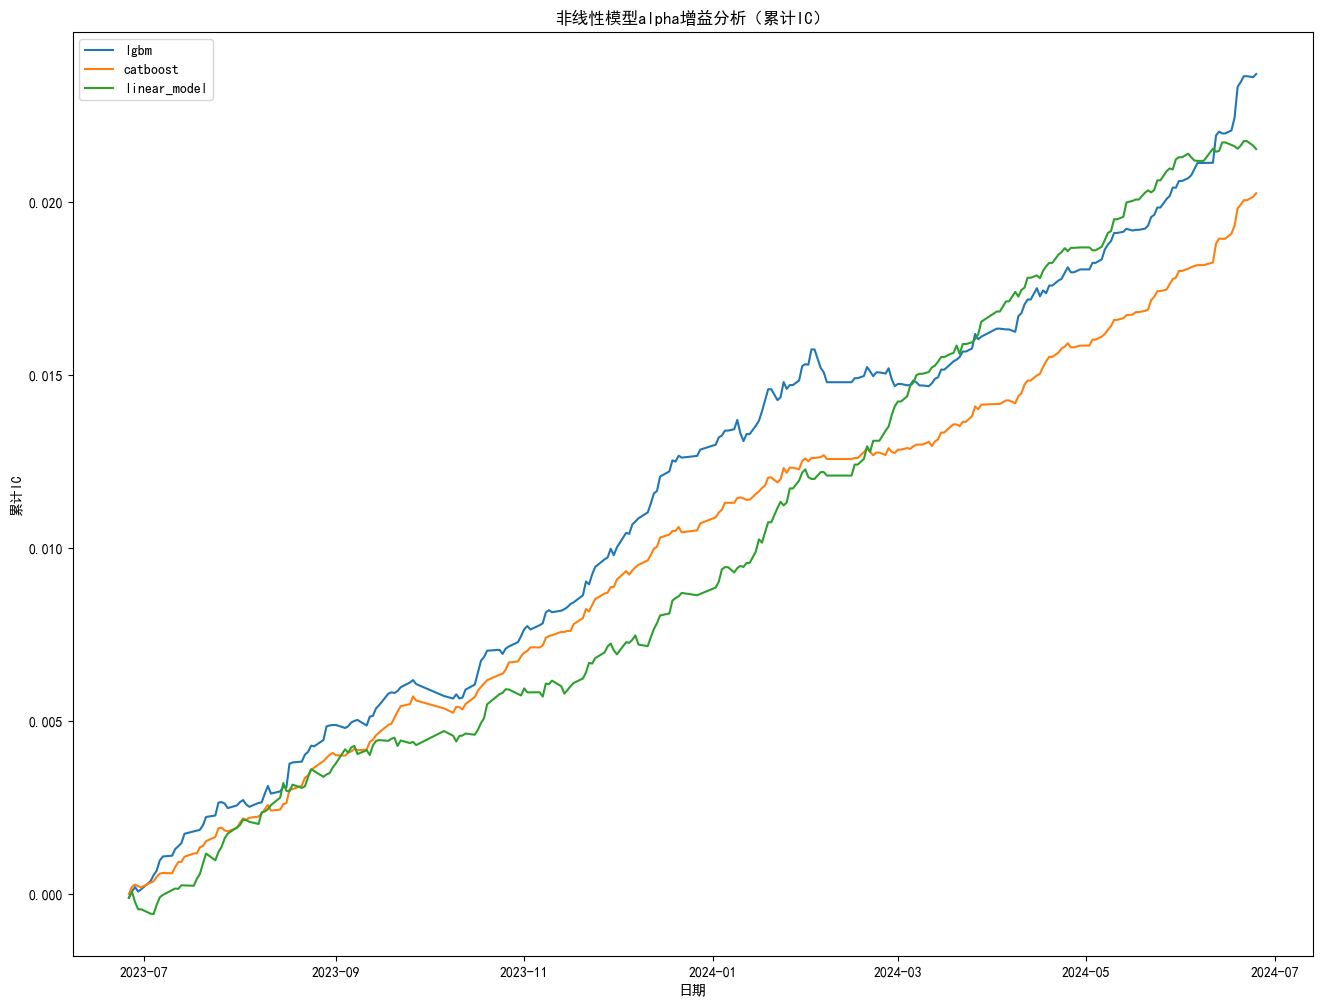
\includegraphics[width=\linewidth]{non-linear-outofsample.png}
{\scriptsize 图：样本外IC对比——线性 vs 非线性模型}
\end{columns}
\end{frame}

% ======================== 第五部分：总结 ========================
\section{总结与展望}

\begin{frame}{总结：北向资金的"双刃剑"效应}
\textbf{学术贡献}
\begin{enumerate}
    \item 北向资金具备显著超额收益（$t=3.82$），以\textbf{择时}为主（58\%）。
    \item 交易模式为"对冲基金式"高频交易，预测力\textbf{仅限短期}。
    \item 净流入引发约\textbf{一周}的市场羊群效应。
    \item \textbf{首次}以DID方法识别出沪港通标的股波动率系统性上升的因果效应。
    \item $\Rightarrow$ 北向资金对A股价格发现功能贡献有限，高频交易\textbf{加剧短期波动}。
\end{enumerate}

\vspace{0.3em}
\textbf{工业贡献}
\begin{enumerate}
    \item 提出"类Barra"残差化框架解决A股虚假动量alpha问题。
    \item 线性模型实现年化14.5\%超额收益、夏普比$\approx$5.0的高质量alpha。
    \item 非线性模型未带来增益$\Rightarrow$线性结构为当前alpha主成分。
\end{enumerate}

\vspace{0.3em}
\textbf{未来方向}：扩展深港通分析 $\cdot$ 引入更多异质性数据源 $\cdot$ 精细化交易成本评估 $\cdot$ 探索中间模型形式（GAM等）
\end{frame}

% ======================== 致谢 ========================
\begin{frame}
\centering
\vspace{2cm}
{\Huge\bfseries 谢谢！}

\vspace{1.5cm}
{\large 欢迎提问与讨论}
\end{frame}

\end{document}
